\cleardoublepage
\chapter{DOKUMENTASI KOORDINASI PENGADAAN (WAWANCARA 3)}
\label{chap:lampiran_c}

\section{Dokumentasi Foto Wawancara 3}
Berikut adalah dokumentasi visual pada saat koordinasi teknis mengenai instalasi perangkat keras di area lobi dan basemen.

\begin{figure}[htbp]
    \centering
    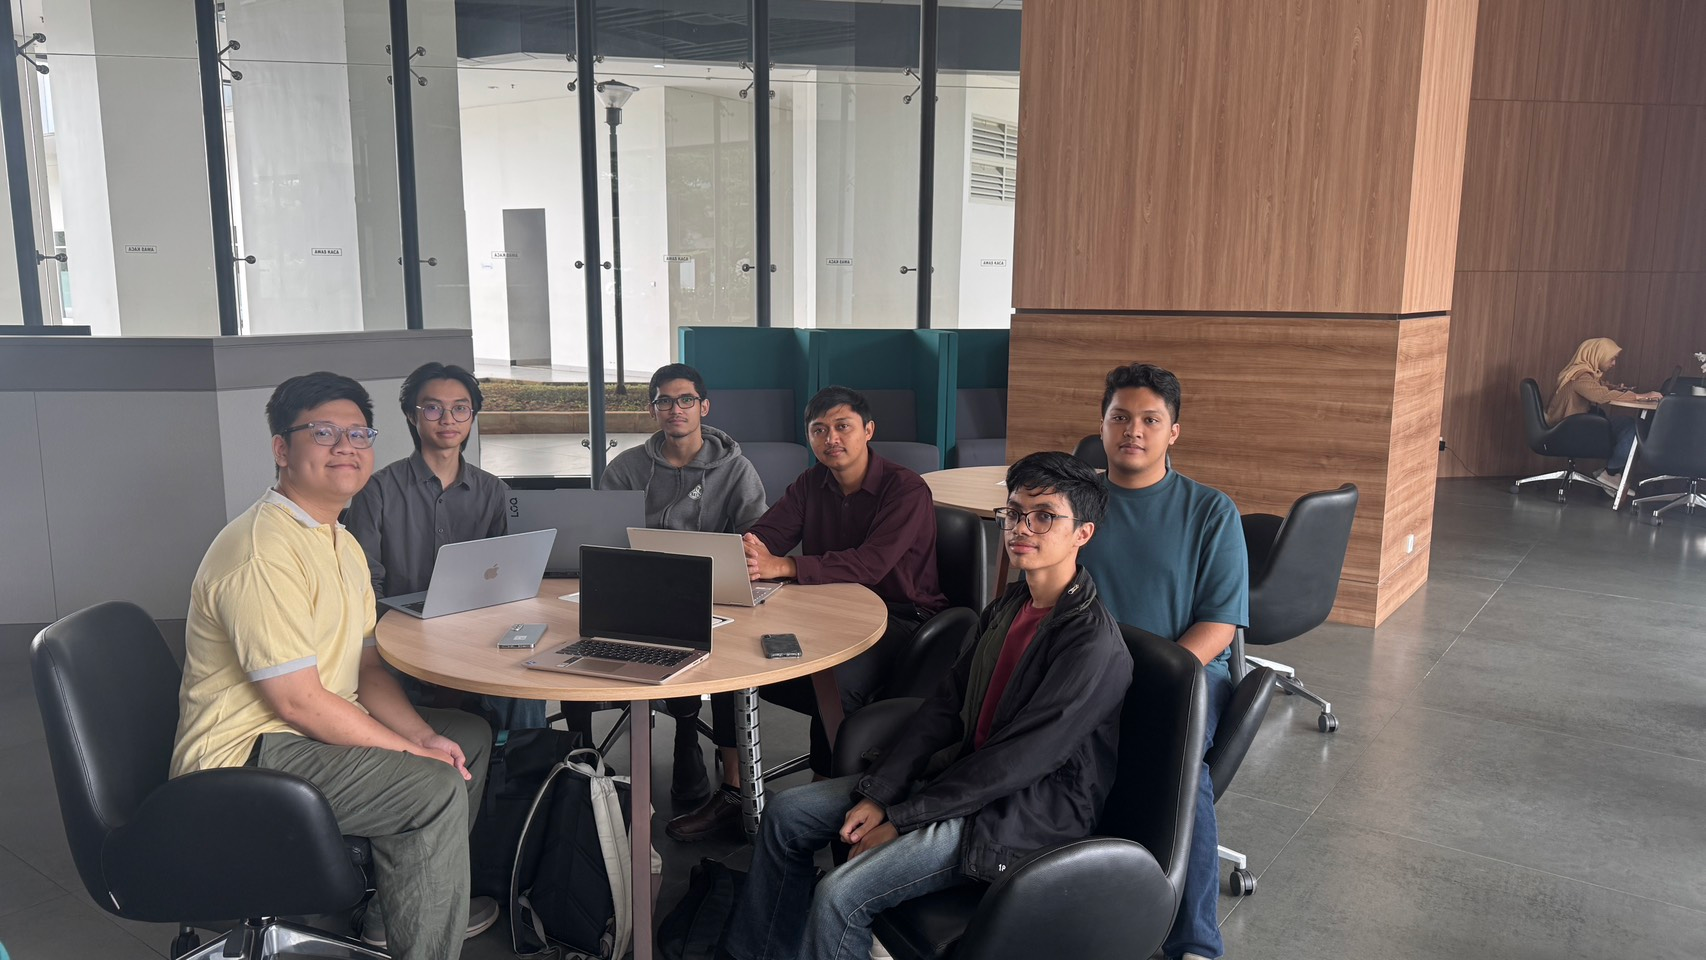
\includegraphics[width=0.6\textwidth]{images/wawancara3_1.png}
    \caption{Koordinasi Lapangan 1}
\end{figure}

\begin{figure}[htbp]
    \centering
    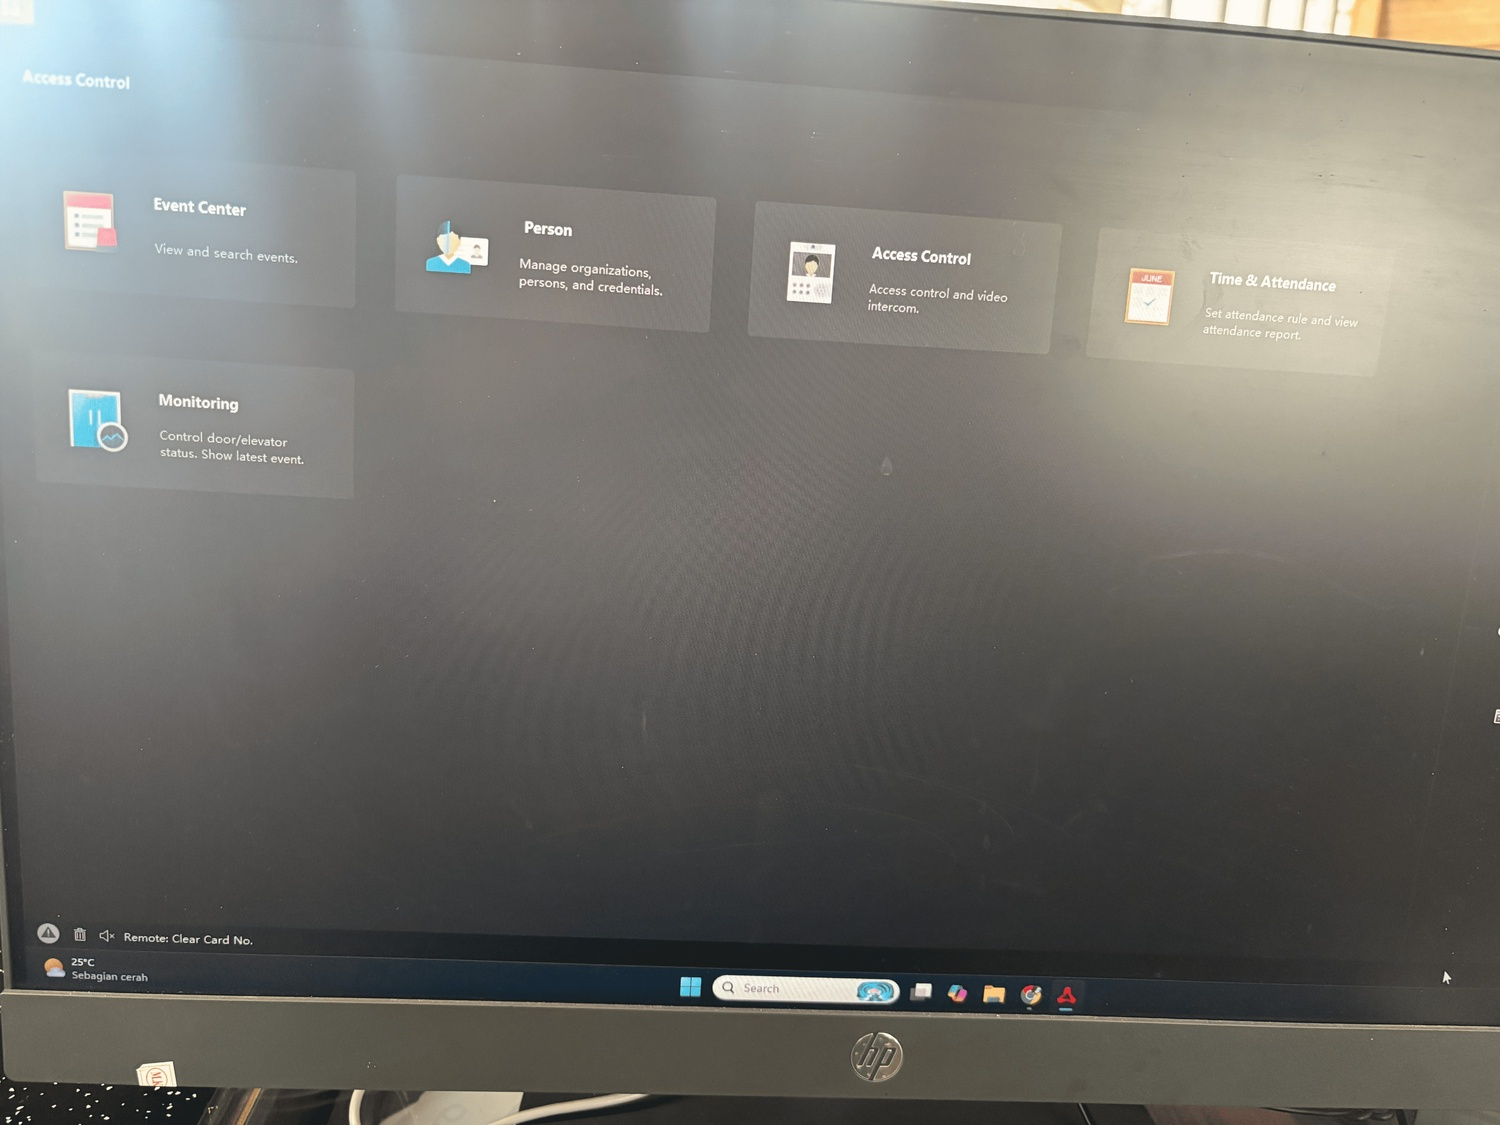
\includegraphics[width=0.6\textwidth]{images/wawancara3_2.png}
    \caption{Koordinasi Lapangan 2}
\end{figure}

\begin{figure}[htbp]
    \centering
    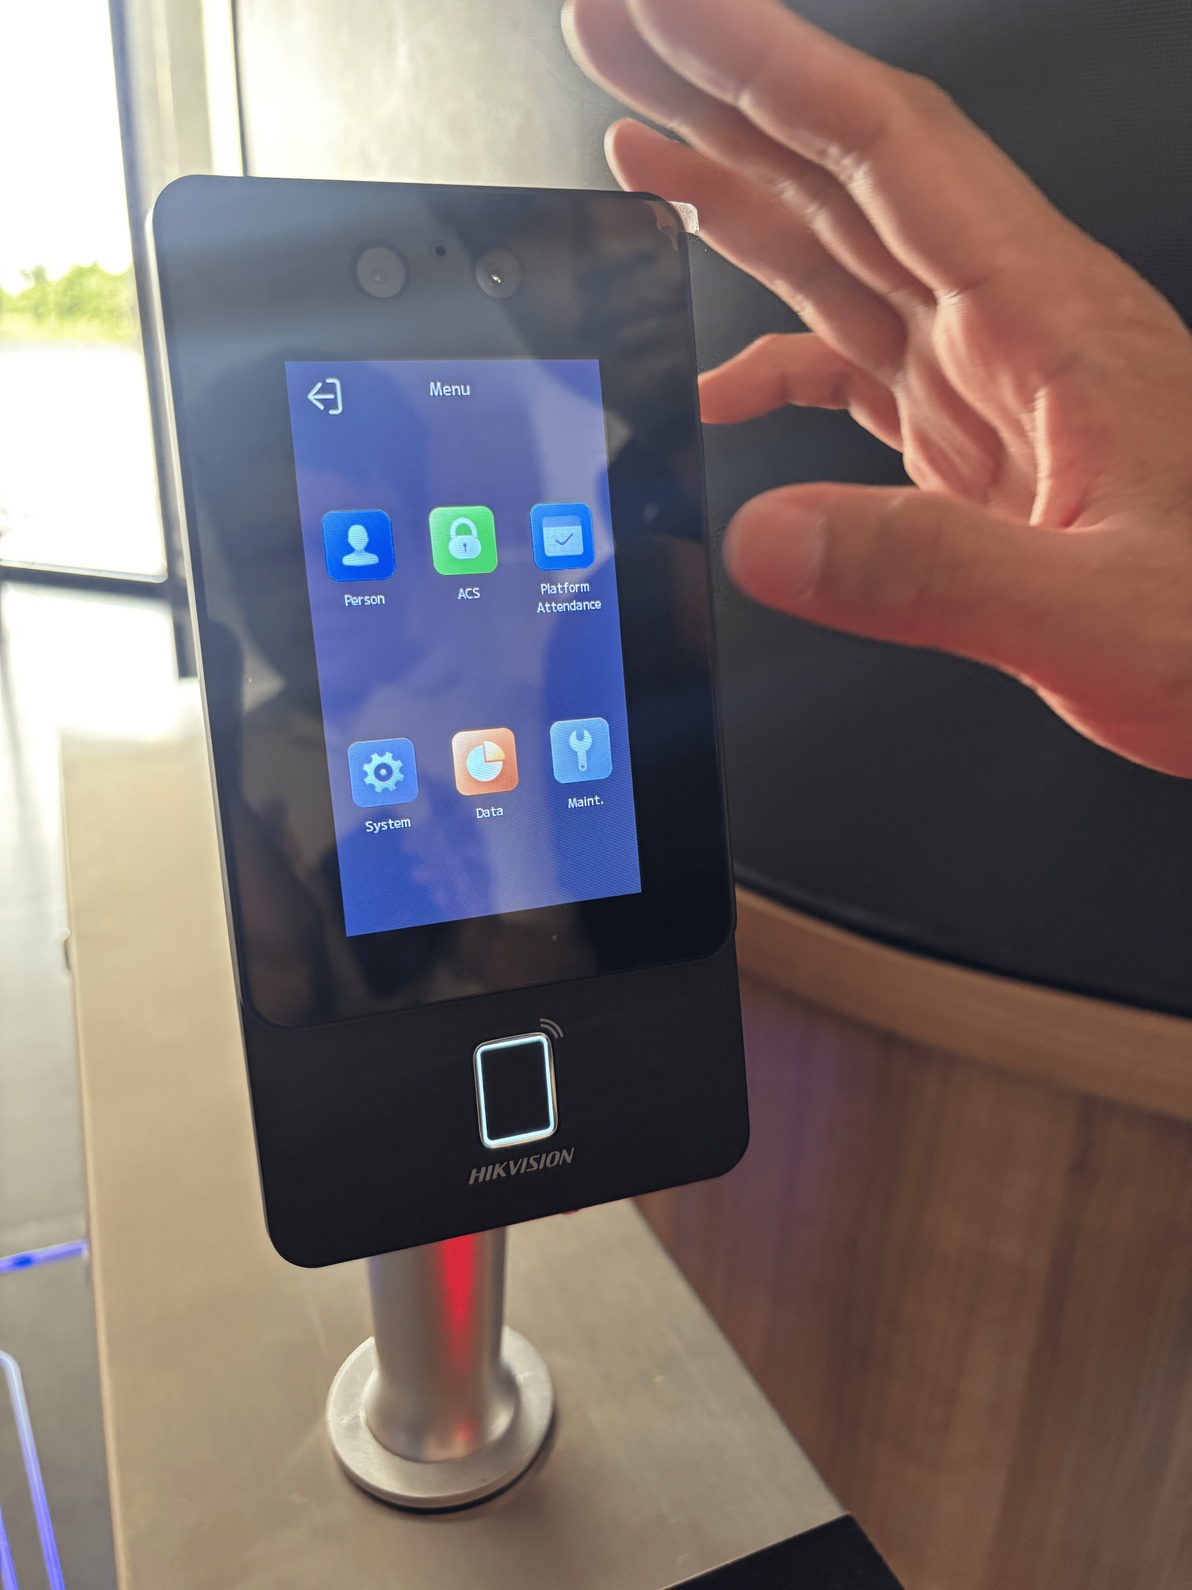
\includegraphics[width=0.6\textwidth]{images/wawancara3_3.png}
    \caption{Koordinasi Lapangan 3}
\end{figure}

\begin{figure}[htbp]
    \centering
    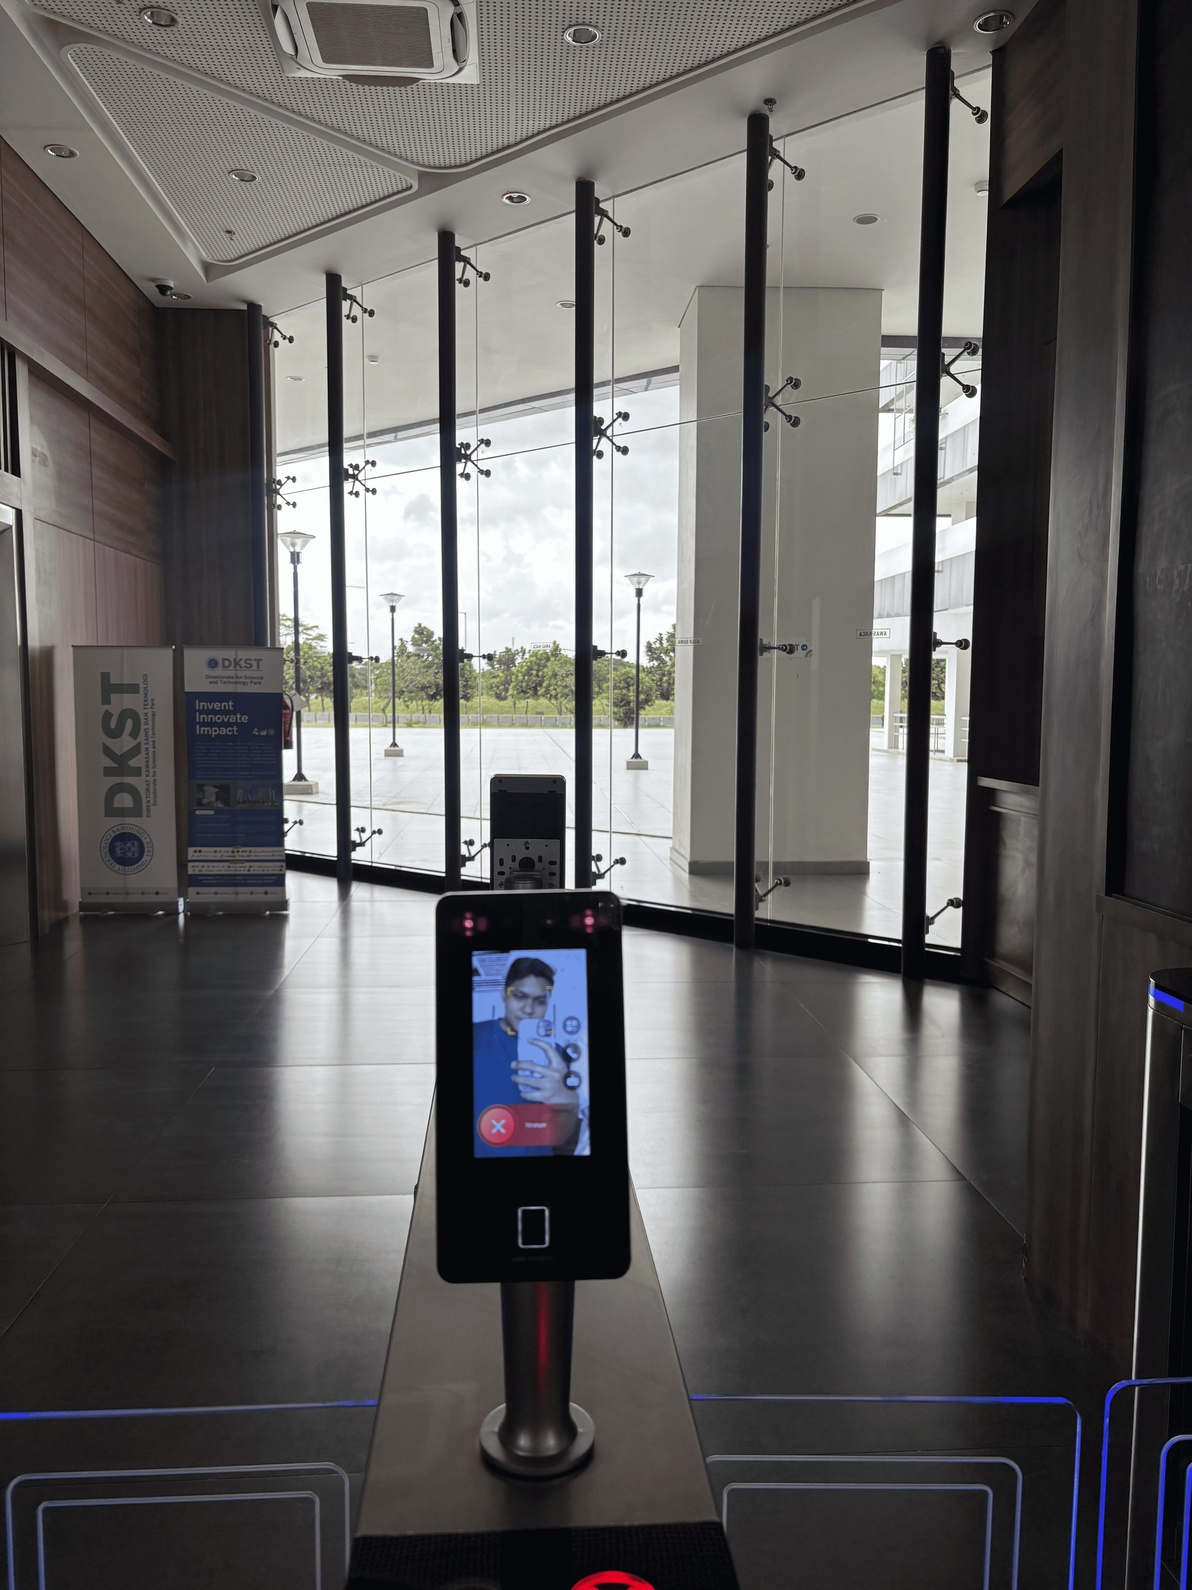
\includegraphics[width=0.6\textwidth]{images/wawancara3_4.png}
    \caption{Koordinasi Lapangan 4}
\end{figure}

\section{Transkrip Wawancara 3}
Wawancara ketiga dilakukan bersama Kepala Seksi Data \& SI DKST untuk membahas detail integrasi \textit{Building Management System} (BMS), sistem absensi, dan kebijakan keamanan data di lingkungan ITB. Berikut adalah transkrip lengkap dari diskusi tersebut:

\begin{longtable}{|c|p{0.35\textwidth}|p{0.55\textwidth}|}
\hline
\textbf{No} & \textbf{Pewawancara (Mahasiswa)} & \textbf{Narasumber (Kepala Seksi Data \& SI DKST)} \\ \hline
\endfirsthead
\hline
\textbf{No} & \textbf{Pewawancara (Mahasiswa)} & \textbf{Narasumber (Kepala Seksi Data \& SI DKST)} \\ \hline
\endhead
\hline
\endfoot
\hline
\endlastfoot
1 & Terkait fitur absensi dan pelacakan, apa ekspektasi Bapak dari sistem yang akan dibangun? & Sistem harus bisa melacak kehadiran dan lokasi orang secara akurat (masuk jam berapa, terakhir keluar jam berapa). Ini penting karena di ITB ada insentif kehadiran yang bisa dipotong jika absen tidak terekam dengan baik karena telat atau sistem \textit{error}. \\ \hline
2 & Untuk sistem kamera pengawas, fungsionalitas apa yang menjadi prioritas Bapak? & Prioritasnya adalah menghitung jumlah orang yang keluar masuk, mengetahui lokasi spesifik seseorang (misal: apakah dia sedang di ruang rapat), serta mendeteksi wajah asing/baru untuk keamanan. Deteksi orang lebih diprioritaskan dibandingkan deteksi bahaya fisik. \\ \hline
3 & Bisa dijelaskan sedikit mengenai peran DKST di Gedung IIP ini? & DKST memiliki 4 fungsi: 1. Transfer teknologi (Paten/HAKI), 2. Inkubasi bisnis/startup, 3. Inovasi riset, dan 4. Pengelolaan kawasan (sewa \textit{coworking space}, ruang rapat, kantor). Proyek TA kalian ini sebenarnya bisa dimasukkan ke program inkubasi bisnis kami untuk mendapat pendanaan. \\ \hline
4 & Bagaimana sistem absensi karyawan DKST saat ini berjalan? & Karyawan tetap terpusat di sistem ITB, sedangkan pegawai kontrak (TAD) absennya terpisah. Saya membuat sistem internal agar absen TAD terpantau untuk keperluan insentif. Kendala saat ini adalah gerbang \textit{basement} tidak bisa mendeteksi orang saat keluar, jadi riwayat pergerakannya terputus. \\ \hline
5 & Terkait integrasi \textit{Building Management System} (BMS), apakah perangkat di gedung ini sudah saling terhubung? & Belum ada sistem terpusat. Sistem gerbang, kamera, dan AC masih terpisah dengan aplikasi vendornya masing-masing. Harapannya, sistem yang kalian buat bisa menyatukan pemantauan tersebut dalam satu \textit{dashboard} web terpusat agar petugas tidak perlu membuka banyak aplikasi. \\ \hline
6 & Bagaimana alur pendaftaran dan sinkronisasi data pada \textit{software} bawaan vendor saat ini? & Pendaftaran wajah/kartu dilakukan di satu mesin, lalu datanya di-\textit{get} ke aplikasi \textit{desktop}, baru didistribusikan ke mesin lain. Pernah kejadian data hilang karena sinkronisasi saling menimpa (\textit{overwrite}). Harapannya \textit{middleware} kalian bisa mengotomatisasi ini tanpa bergantung pada aplikasi \textit{desktop} bawaan. \\ \hline
7 & Apakah ada fitur notifikasi \textit{real-time} yang diharapkan untuk audit keamanan? & Akan sangat bagus jika sistem bisa mengirimkan notifikasi instan ke WhatsApp (lebih efisien daripada \textit{email}). Misalnya, jika ada wajah asing terdeteksi masuk lobi, sistem otomatis memotret dan mengirimkan fotonya ke grup WhatsApp petugas keamanan. \\ \hline
8 & Untuk kebutuhan pengujian (\textit{testing}), apakah kami diizinkan untuk mengakses perangkat NVR dan kamera secara langsung? & Boleh, silakan buat surat permohonan resmi untuk izin akses ke satu alat NVR dan kamera untuk riset. Namun harus sangat berhati-hati, karena jika kalian salah memasukkan \textit{password} 5 kali berturut-turut, sistem NVR akan terkunci (\textit{lock}) dan perangkat harus dikirim ke pabrik untuk di-\textit{reset}. \\ \hline
\end{longtable}
